The lunar farside provides a uniquely accessible RF environment in that the moon shields it from Earth and near-Earth RFI at all times. Therefore, {\em anything} detected there is of scientific interest. Since there is no ionospheric blockage, low-frequency observations that are impossible from Earth can also be made in this RFI-free environment. Although the lunar farside will remain an excellent low-RFI site for many years to come, {\em now} is the only time to take completely pristine measurements of the radio spectrum. This is an opportunity that will never again present itself, as seen in Fig.\ \ref{fig:missions}.  This section summarizes the primary science cases that drive the design of the array, which is summarized in the science traceability matrix in Appendix A.

\subsection{Technosignatures}
Humanity's quest to determine its place in the Universe and whether we are its only inhabitants has driven our imagination and quest for knowledge since we first looked to the sky.  Designs for many large telescopes are being considered to help determine if other biological processes are happening among nearby stars (called "biosignatures").  We now also have the capability to explore whether technological signals (``technosignatures'') exist over a large swath of our Galaxy.  The Breakthrough Listen program has transformed the field and has greatly expanded the search for such technosignatures (e.g. \citealt{Enriquez_2017, Price_2020, Gajjar_2021}).  The greatest impediment to this program is the prevalence of RFI made by essentially every device on Earth that is electrically powered.

Although RFI is prevalent, excellent technosignature searches can be conducted from the earth, particularly from remote locations where terrestrial interference is low and in frequencies that, at that time, place and frequency, are free of interfering signals. See Figure \ref{fig:bubbles} where the circles represent the ground-based radio searches that have been done and the highlighted regions of two of the large program (purple and red shaded regions) technosignature searches in progress. In order to further guard against temporary interference, one usually uses a cadence of a series of on-targets and off-targets, where the ``off'' can be the ``on'' for another target. The use of this in a multi-beam system as outlined in Figure \ref{fig:midband_beam_maps} is demonstrated in \cite{Huang_2023}. Note that using a multi-beam system allows for the ``on'' and ``off'' to be simultaneous, making it even more efficient (i.e., \citealt{multibeam}). A significant amount of detection time is, however, highly desirable. Also, note that a remote site doesn't provide shielding from satellites and airplanes. Techniques do exist to subtract or decorrelate interference, however they are not perfect and it seems unlikely that a technosignature detection ``through'' RFI would be believed -- even if not immediately rejected in a pipeline, as would likely be the case.

\begin{figure}
    \centering
    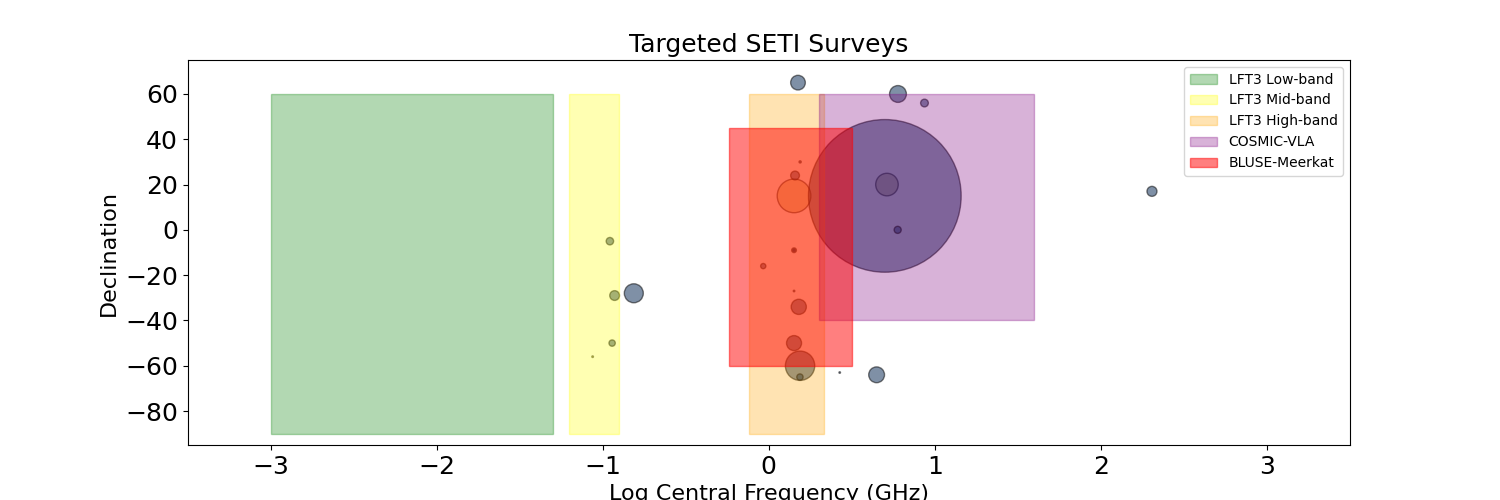
\includegraphics[width=0.85\linewidth]{SETI_Bubble_LFT3.png}
    \caption{A plot of the historical technosignature searches modified from \cite{Tremblay_2022}. The circles size is scaled to the total number of targetted sources within the survey. The colored rectangles show the regions in frequency and declination that LFT3 will cover as well as two large ground-based programs. As shown, LFT3 will survey regions that cover both new or rare regions (low and mid bands) as well as well studied regions (high-band).}
    \label{fig:bubbles}
\end{figure}

Of course, we don't have any information on any parameter of a technosignature, so one must search agnostically with the most sensitive receivers one can muster.  However, we do know that the most likely initial signal detected will have a high signal-to-noise in some parameter space. For now, at radio wavelengths, that parameter space is frequency space and narrow-band signals are the most likely to be detected.  Additionally, they are among the least likely signals to be confused with an astrophysical process. There is a case to be made, that the most likely initial detection will be a slow transient arising from some underlying cadence such as a civilization targeting many distant worlds with a beacon or some fortuitous alignment such as the conjunction of two extrasolar planets with our telescope beam.  As mentioned in the Introduction, the ``Wow!'' signal is an exemplar of what one such signal could look like.  As also mentioned, if observed from the earth even if that event occured where it wasn't obscured by RFI one would likely not have a high confidence of its origin due to the many other sources of potential short-term RFI. To reliably detect such a signal one must go to a place with no other potential sources.

In order to assess if a small telescope can meaningfully search for technosignatures it is instructive to look at detectability of various transmitter strengths for the stellar distribution around us. The Arecibo planetary radar has been the highest effective isotropic power radiator at a level of greater than 20 TW and is a key fiducial. Another is to assume that an advanced civilization could produce significantly greater radiated power, in this case we will use 1000 times the Arecibo planetary radar.  Figure \ref{fig:isaacsonetal} shows the signal-to-noise ratios if these transmitters were at the location of stars in various star catalogs.  As shown, even our current technology provides a detectable signal to this telescope.

\begin{figure}
    \centering
    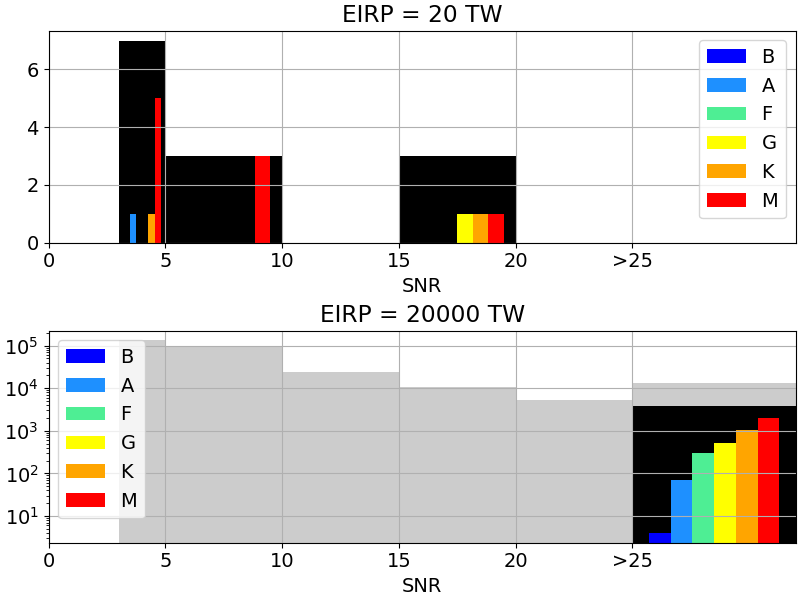
\includegraphics[width=0.75\linewidth]{figures/catcounts.png}
    \caption{Detection counts for the Breakthrough Listen target selection for nearby stars \citep{2017PASP..129e4501I} and a catalog of stars within 100 light years (https://chview.nova.org/solcom) for an ``Arecibo'' scale transmitter (top) and 1000 times larger (bottom).  The black background is the total number per signal-to-noise ratio bin and the colors are the individual spectral types.  The first bin extends from 3-5 and the last bin is 25 and greater.  The light gray on the bottom plot shows the shows the same calculation for all of the stars in the Gaia Nearby Start Catalogue \citep{2021A&A...649A...6G}}
    \label{fig:isaacsonetal}
\end{figure}

% Paragraph below is now redundant.
% Signals of interest must be carefully sought within this cacophony of RFI. To differentiate between RFI and a technosignature requires that the technosignature signal is at a frequency/time not inhabited by RFI and the signal must persist and be quite stable over a timeframe of many minutes.  The signals are assumed to be nearly monochromatic and slow-drifting in time.  A series of on-off measurements are used (for single-dish experiments)to make sure that the signal-of-interest is coming from the main beam of the telescope and not RFI in a distant sidelobe.  These techniques are incredibly powerful in conducting senstive searches over the available bandwidth, and have the added benefit being able to use very large earth-based telescopes to dramatically increase the sensitivity.  However, many limitations exist on appropriate ranges of frequency and time, and some frequency ranges are so impacted that searches (and radioastronomy research generally) are infeasible in those bands.  Signals of short duration (a few seconds) or signals heavily modulated are nearly impossible to discern.  And of course, technosignatures ``behind'' RFI is not detectable (or at least believably so).

\begin{figure}
    \centering
    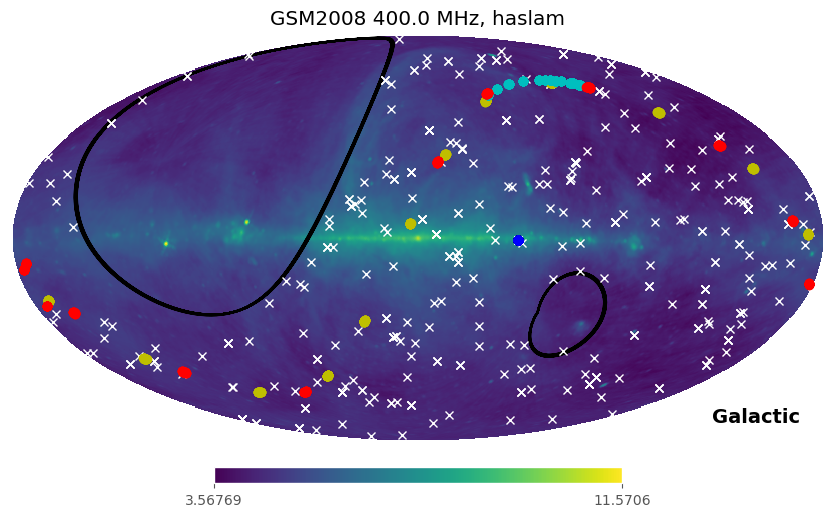
\includegraphics[width=0.95\linewidth]{figures/galaxy_plot.png}
    \caption{Graphic showing the field-of-view of LFT3 over a month imposed over a graphic of the Milky Way at 650 MHz.  The white `*'s are all of the stars within 10pc within the field-of-view, the blue dot is Alpha Centauri, the yellow dots are the Sun at various times over the year 2028, red dots are Mars over that period and the cyan dots are Jupiter.}
    \label{fig:fieldofview}
\end{figure}

%With online beamforming capabilities we can search the nearest stars  across a range of frequencies rarely searched from Earth but represent some of our most power transmitters \citep{Tremblay_2022}. Within the current FPGA framework, calibration and dynamic spectrum creation can be completed giving us access to the full details of the signals detected for each frequency range. This combined with a sample of the time-averaged spectrum will provide a unique dataset in which to seek an answer to ``Are we alone?". Assuming a civilization is capable of building a big dish to generate an isotropically distributed signal of $\sim$10${^17}$\,W, with a 6$\sigma$ sensivity of 0.5\,Jy, we could expect to detect that signal out to about 3\,pc. However, a beamed signal or a large megastructure is expected to create power over 10$^{26}$\,W. 

%The $Gaia$ Space telescope has given has a large catalog of targets which we are already using in blind, commensal surveys with MeerKAT (Czech et al. in prep) and the Karl G. Jansky Very Large Array \citep{Tremblay_2024}. From this experience we can develop and efficient search working on the FPGA framework.

\textbf{Science Specifications:} As shown in Figure \ref{fig:bubbles}, the proposed telescope frequency covers a new parameter space in technosignature searches, especially with the low- and mid-band receivers. The technosignature science case requires some in-line processing of the data to find signals of interest and generation of dynamic spectra or raw voltage postage stamps around signals of interest. On the commensal, real-time system at MeerKAT and the VLA \citep{Tremblay_2024} we use \textsc{seticore}\footnote{\url{https://github.com/lacker/seticore}} to search for the signals toward beamformed targets. \textsc{seticore} uses an efficient Taylor-Tree dedispersion algorith to autonomously search for narrowband signals. The user specifies the signal-to-noise ratio to identify signals of significance and the drift rate search width. To save on information needing to be transfered to the ground, instead of sending the dyanmic spectrum, we can de-disperse the signal and only transmit the time averaged power spectrum. 

As there is no known signal thus far identified, the frequency resolution and time resolution are open parameters that are flexble to needs to keep data rates and processing to a minimum. However, most of current radio astronomy experiments utilize $<$10\,Hz frequency resolution. 

We can verify these modes of operation by looking toward Mars where there are number of space-based and ground-based communication signals heading back to Earth on a regular basis. The carrier signals are often emitted at around 2\,GHz and represent a population of narrow-band artificial signals.

\subsection{Transients}
The recent flourishing of the field of radio transients (both slow and fast) has brought a wealth of information, significantly advancing various areas of physics. Notably, pulsars and fast radio bursts (FRBs) stand out due to their unique potential to reveal new kinds of physics. These astrophysical phenomena offer valuable insights into gravitational waves, cosmology, and plasma physics, among other fields. However, beamforming radio observations can also shed light on other transients such as flare stars and planetary conditions within and outside the solar system. Overall, the strength of a lunar-based telescope is in discovering the unknown. This could include the possible detection of various “low-DM” (or dispersion measure, an indicator of relative proximity) events, on timescales of milliseconds to minutes: low-DM FRB analogues, FRBs from galactic magnetars, decimetric solar bursts, stellar bursts, and undiscovered time-domain phenomena. In particular, the discovery of new populations of transient astrophysical sources in the very local Universe.

\begin{figure}[!ht]
    \centering
    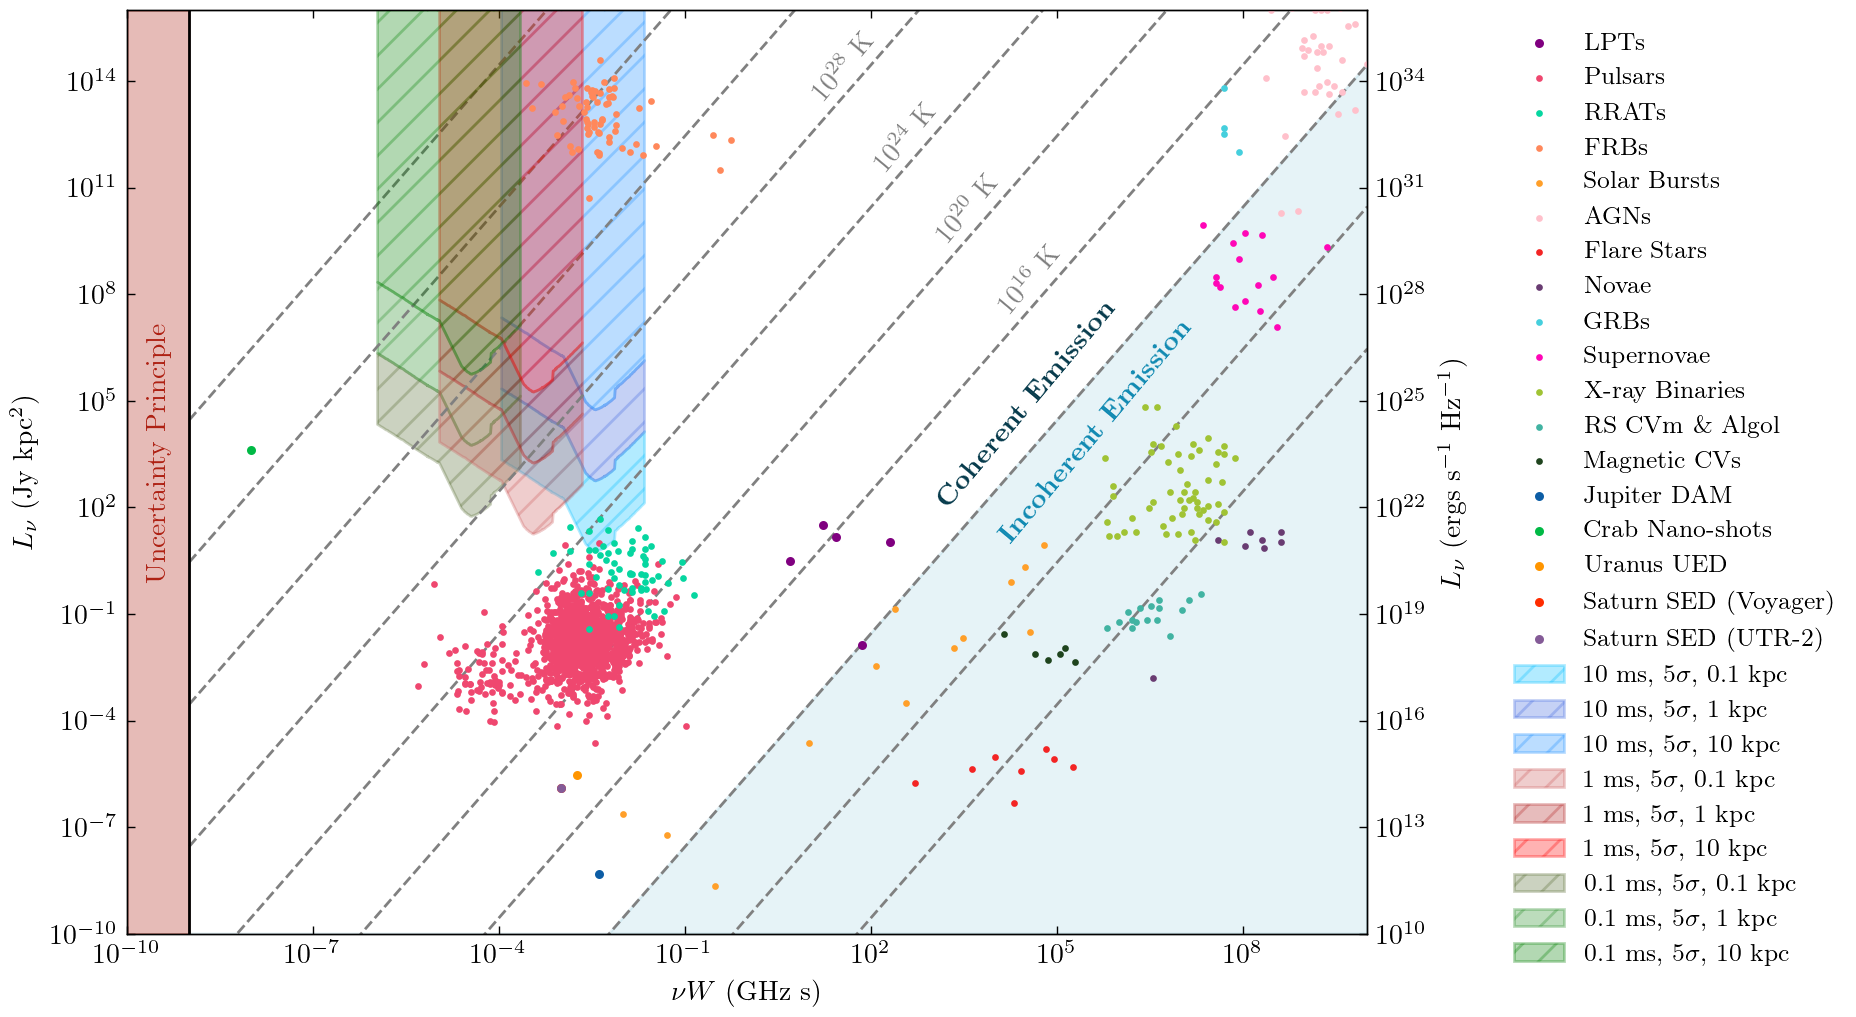
\includegraphics[width=0.8\textwidth]{figures/phase_space.png} % Placeholder image
    \caption{Transient Parameter Space figure adapted from \citet{pietka}. This plot illustrates the sensitvity regions of a LFT3 obsevrational setup across differnt pulse widths (0.1~ms, 1~ms and 10~ms) on a $\nu \text{W}$ vs. $L_\nu$ phase diagram. Where $\nu \text{W}$ represents the product of observed frequency and pulse width and $L_\nu$ shows the spectral luminosity. The the blue, green and red hashed regions correspond to a pulse width and show the detectable signal levels above a threshold of $5\sigma$ for the LFT3 bandwidth.}
    \label{fig:placeholder}
\end{figure}

\subsubsection{Pulsars}
Pulsars are highly magnetized, rotating neutron stars that emit beams of electromagnetic radiation. Pulsars serve as precise cosmic clocks, providing insights into the interstellar medium, gravitational waves, and the fundamental physics of matter under extreme conditions. It is theorized that pulsars spin rapidly upon creation and slow down due to gravity over time, along with changes in the medium surrounding the pulsar, which alters the pulse structure as well \citep{LW_2013}. By using coherent beamforming, sensitivity to weak pulses can be improved, and frequency and time resolution can be adjusted to decrease the effects of dispersion measure smearing (e.g. \cite{WL_2020}).

Broadband studies of pulsars allow for a study of the emission physics and surrounding material, where the lower frequencies are sensitive to emission closer to the pulsar surface. With ground-based radio telescopes, the ionosphere can create challenges, especially in weaker pulsars that have a peak spectral turn-over between 100--200~MHz \citep{Stappers_2011}. By moving the radio telescope off the Earth, away from the ionosphere cut-off around 30~MHz, a broader range of pulsar emission physics can be studied than has not yet been explored. One of the lowest pulsar detections was observed with the Low Frequency Array detecting emission down to 15~MHz \citep{Kondratiev_2012}. LFT3 could be well placed to observe some of the brightest pulsars below 15~MHz. 

A farside lunar telescope, shielded from Earth’s radio frequency RFI, would significantly enhance pulsar observations by providing a pristine observational environment. This location allows for low-frequency studies, critical for understanding the early stages of pulsar emission mechanisms and the surrounding interstellar medium. Furthermore, the lunar farside offers an opportunity to continuously monitor pulsars without the interruptions caused by the Earth’s rotation, increasing the data quality and allowing for the detection of subtle changes in pulsar behavior over time.

To improve the precision of pulsar timing arrays (PTAs), it is essential to address diurnal systematic errors that arise due to Earth's rotation. \textbf{CL: is this a dominant error? I'm surprised, is there a reference?} By calibrating this daily noise factor using the Vela pulsar, one of the brightest and most stable pulsars, a correction model can be developed that enhances the accuracy of timing measurements across the array. This calibration on Vela can serve as a reference for mitigating similar systematic errors in other pulsar observations, thereby refining the overall data quality of PTAs and LFT3 would be in an ideal position to do this. 

\textbf{Science Specifications:} Beamformed data products are highly valuable for discovering a wide range of transient events, with pulsars being one of the key beneficiaries. LFT3 will provide extensive sky coverage, particularly at lower frequencies, which results in a lower effective area $(A_{\text{eff}})$. Consequently, the pulsar candidates identified by LFT3 are more likely to be giant pulses observed at unique frequencies. However, the ability to observe pulsar emissions in a pristine environment across a large bandwidth holds significant scientific value on its own. 
%LFT3 can be compared to instruments like Galactic Radio Explorer \citep[GREX;][]{GREX} which is designed to detect FRBs and Magnetar Bursts. 


% Some known pulsars are so bright and regular that even the simplest setups could detect them. However, for a blind survey of potentially irregular or rare pulsar emission within the inocoherent beam takes a bit more processing. 

% There is a need for a folding mode for the pulsars and the mode can be tested on bright, known sources. This is to test our ability for precise time-keeping and can be verified with ground-based telescopes.

% \begin{figure}[h!]
%     \centering
%     \begin{subfigure}[b]{0.44\textwidth}
%         \centering
%         \includegraphics[width=\textwidth]{example-image-a}
%         % \caption{Caption for Figure 1}
%         \label{fig:fig1}
%     \end{subfigure}%
%     \begin{subfigure}[b]{0.44\textwidth}
%         \centering
%         \includegraphics[width=\textwidth]{example-image-b}
%         % \caption{Caption for Figure 2}
%         \label{fig:fig2}
%     \end{subfigure}
%     \caption{Pulsar Senstivity Plots}
%     \label{fig:sidebyside}
% \end{figure}


\subsubsection{Fast Radio Bursts and analogues}
Fast Radio Bursts (FRBs) are intense, millisecond-duration radio pulses originating from extragalactic sources. Their origins remain one of the most intriguing mysteries in modern astrophysics. Although Galactic magnetars have shown to exhibit similar FRB-like emission \citep{BC_2020,chime2020sgr1935}, the exact progenitors and emission mechanisms are still unknown. Some bursts are observed from stellar environments which show evidence for recent star formation activity, e.g.~\citet{piro2021}. The stellar environments of other sources such as FRB 20200120E suggest that FRB progenitors may emit bursts long after star formation activity~\citep{kirsten2022m81} has ended, providing evidence for multiple formation channels.

The Canadian Hydrogen Intensity Mapping Experiment (CHIME) telescope is currently the world leader for detecting new Fast Radio Bursts with its 200\,deg$^{2}$ field-of-view and observing frequency of 400--800\,MHz, and outrigger stations for burst localization~\citep{leung2021synoptic,lanman2024kko}. 

Where a low-frequency Lunar telescope can provide a large benefit, is in understanding the true nature and populations of FRBs is through the study of emission at lower radio frequencies with high time resolution, as this is becoming a clear factor in understanding the source populations. \textbf{CL: I would add that widefield ground stations, which would likely be built as engineering pathfinders, could co-observe and offer the unique opportunity to pinpoint and study a bright, local FRB with micro-arcsecond resolution. Like in the case of FRB 20200120E, the unique combination of high angular resolution and a nearby source offers the greatest insight into the origins.}

Currently, the Commensal Real-time ASKAP Fast Transients Collaboration (CRAFT; 700--1.8\,GHz) offer the largest number of localized repeater sources \citep{SM_2023} \textbf{CL: Sherman et al. is a DSA-110 paper - I think you actually want~\citep{shannon2024ics} and~\citep{SD_2023} as you put further down below}, with some more recent contributions from the Five-hundred-meter Aperture Spherical Telescope (FAST) collaboration \citep[1.00--1.45\,GHz;][]{ZX_2023}) and the DSA-110 \citep{LC_2023,sharma2024preferential}. The missing gap in understanding the true nature and originating source of emission is observing away from the influence of RFI and away from the ionosphere.

Low-frequency observations of FRBs are crucial for understanding their propagation through the intergalactic medium, potentially unveiling the distribution of baryonic matter and offering clues about the emission mechanism and source plasma environments. LOFAR observations of FRB 20180916 have revealed potential evidence for interaction between a neutron star and its binary companion by observing bursts down to 100 MHz~\citep{pleunis2021lofar}. A farside lunar telescope, free from RFI and ionospheric distortion, would enable unprecedented low-frequency observations, shedding light on FRB origins, propagation effects, and contributing significantly to the broader understanding of cosmic phenomena.

\textbf{Scientific Specifications:} Given the values shown in Figure \ref{fig:freqbands}, we calculated the expected sensitivity to FRB emission. If we assume 20\,seconds of integrated time for a de-dispersed signal at a bandwidth (BW) of 100\,MHz, then we would have a 5\,$\sigma$ flux density limit of 10--11\,Jy over an incoherent sum. The CHIME telescope evaluated 25 repeating FRBs and found them to have 63\,ms of peak widths with bandwidths of 50-200\,MHz \citep{CHIME_RepeatingFRB}. Therefore, we would need a time resolution of $<$1\,ms. However, they found the dispersion measures (DMs) to range from 220 to 17,000\,pc\,cm$^{-3}$ meaning we would need the compute capacity to run through this range to identify blind candidates. 

Most sources had the strongest emission at 400--600\,MHz, suggesting we would only need to do this experiment with one set of dipoles. The CHIME experiments have a sensivity limit of 0.339\,Jy, suggesting that with a limit of 11\,Jy it would be challenging to find new sources of emission from extragalactic-FRBs. An increase in bandwidth or time would add a $\sqrt{BW\times\tau}$ increase in sensitivity, where $\tau$ is the total integration time in seconds and BW is in Hz. \textbf{There also exists a nascent population of Galactic ``long-period radio transients''~\citep{hurleywalker2022radio} detectable at lower dispersion measures.} In either scenario, a de-dispersed dynamic spectrum would be the most compressed output for sending to Earth for further analysis.

\textbf{CL: It is possible to estimate the FRB rate from CHIME, which detects about 1000 bursts per full year of observation in the same frequency range over a 200 deg$^2$ FoV with a coherent SEFD of 50 Jy. Assuming a Euclidean population of sources, in the coherent FoV of LFT3 of $\sim 4000$ deg$^2$ at the bottom of the mid-band, $\sim 0.88-2.5$ bursts could be detected per year of observation.}

\subsubsection{Flare Stars}

Radio flare stars, often young, magnetically active stars, provide insight into stellar magnetic activity, star formation, and the early stages of stellar evolution. Observations from a farside lunar telescope could reveal details about the mechanisms driving these flares and their impact on the surrounding stellar environment. Studying radio flare stars also has implications for exoplanetary science. The intense radiation from these flares can affect the habitability of orbiting exoplanets. \textbf{JT: Flares may also be used to study star-planet interactions.} A farside lunar telescope lends it self to assess the radiation environment of these planets, contributing to our understanding of exoplanet habitability based on the low frequency window observed and the unique RFI enviroment the farside has.

Observing these stars, especially at low frequency ($\leq 300$ MHz) act as probes into stellar and planetary plasma environments. Coronal Mass Ejections (CMEs) have a low-frequency burst component in which information about the kinematics of plasma can be deduced \citep{villadsen_ultra-wideband_2019}. Incident solar wind is also the primary driving force of auroral emission on magnetized planets. Radio emission from stars is typically produced through CMEs, observed phenomenologically in the Sun as type II and III solar bursts. The radio emission from these events is thought to be produced through the electron-cyclotron maser instability \citep[ECMI;][]{EMI}. The ECMI is a plasma instability that occurs in the presence of a magnetic field and a population of energetic electrons. The instability is thought to be the primary driver of radio emission observed in type II bursts and stars as a whole. With type III bursts being thought to be the result of electron beams that are accelerated in the corona.

Emission from planets has also been observed in the form of auroral emission. The most notable example of this is the Jovian system. The Jovian system is known to have auroral emission that is driven by the interaction of the solar wind with the magnetosphere of the planet. Coherent radio emission from the aurora is thought to be produced through the cyclotron maser instability \citep[ECM;][]{zarka_auroral_1998} which injects a high-velocity electron population into the magnetosphere. The maximum frequency of the ECM is directly proportional to the magnetic field strength of the object at its emitting point \citep{kavanagh_hunting_2023, joe_nature_review}.

Much time has been spent observing Ultracool Dwarfs (M7) as they provide a good analogue to the Jovian systems. This allows for direct comparison between the two.  This provides valuable insights into the formation and atmospheric processes. Moreover, such comparative studies contribute significantly to our understanding of planetary evolution and diversity beyond our immediate neighbourhood. Recent detection of radiation belts around a UCD further supports the analogy to Jupiter, as radiation belts are a key characteristic of Jupiter's magnetosphere \citep{joe_nature_review}. \ UCDs, being intermediate in mass between stars and planets, serve as a bridge to understanding exoplanet detection. The discovery of bursting radio emission from a brown dwarf and subsequent detections in UCDs indicate departures from established stellar coronal/flaring relationships. \ Radio bursts from UCDs can exhibit periodic timing \citep{hallinan_rotational_2006} along with strong circular polarization and high brightness temperatures, suggesting the involvement of the ECM process in generating radio emission. Despite a significant amount of gigahertz-frequency radio searches, detection rates for UCD radio emissions remain stubbornly low at around 10\% overall \citep{lynch_radio_2016}. Given that LFT3 will observe from a lunar 



\textbf{Scientific Specifications:} As mentioned flarestars a radio loud on the scale of 10's of mJy's. This puts nearby flare stares well within the relams of detection. As with the other science cases LFT3 allows for observations in previously contamintated or unreachable frequencies, specifcally FM and sub 30~MHz band will be on intrest for monitoring already known bright sources \citep{joe_nature_review}. 


\subsubsection{Solar System Emission} 
There are numerous sources of radio emission throughout the solar system, as already mentioned. Most noteably, Jupiter's strong magnetic field interacts with its moons, in particular Io~\citep{Io} but also Europa and Ganymede~\citep{Corentin}, producing strong megajansky radio emissions \textbf{JT (reword as needed): Jupiter emits from 10 KHz to 40 MHz \citep{zarka_auroral_1998}. Jupiter’s hectometer-wavelength (1-5 MHz) radio emission is controlled by the solar wind \citep{Desch1984}. The benefit of studying Jupiter from the Moon is we will be able study the frequenices that are controlled by the Sun near Solar maximum. This study can also be used as a benchmark for studying exoplanet radio emission from hot Jupiters \citep{Zarka2007,joe_nature_review}. } \textbf{CL: at what frequencies? I would guess this is 10 MHz but could be wrong. Also need to point out that NenuFAR might have seen something but it's challenging from the ground, and that most exoplanets are sub-Neptunes, so it's an interesting region of parameter space.}. A lunar telescope is well-suited to probe low-frequency emissions from the outer solar system planets. During its flyby, Voyager 2 discovered strong $\sim 100$-Jy radio emission from Neptune and Uranus, indicating the presence of strong magnetic fields \citep{zarka_auroral_1998, ZHANG199237}. One particular science case of interet is radio emission from the outer planets Uranus and Neptune. Voyager’s low-band instrument also detected radio emissions associated with lightning storms during its flyby of Uranus. Despite extensive observations by LOFAR and NenuFAR, this particular emission has not been re-detected again since the Voyager flyby \citep{1986Zarka_Emission}. \textbf{JT (edit as need be): We can study lightning from Saturn as well (see \citealt{Zarka2004}) as the emission goes from 2 - 30 MHz and is really bright (1000 Jy). }

\textbf{Scientific Specifications:} Simiarily to the flare star data products dynamic spectra in stokes I and V would be adequate for performing analysis of the morphology of the emission and probing emission polarisation. 

\subsubsection{Exoplanet radio emission and star-planet interactions (added by JT - reduce as needed)} 


 \textbf{Observations of an exoplanet's magnetic field would allow us to holistically understand the planet by providing constraints on difficult-to-study planetary properties. To start, knowledge of a planetary magnetic field can provide robust constraints on a planet's interior structure, including its composition and thermal processes \citep{G2015,Lazio2019,Brain2024}. Historically, initial insights into the interior structure of the Solar System's gas giants were derived from the understanding that they possess magnetic fields \citep{Hubbard1973}. Additionally, magnetic fields will also affect (either enhancing or suppressing) atmospheric escape \citep{G2015,Zarka2018haex,Egan2019,Brain2024}. Magnetic drag could also be an important factor for atmospheric dynamics and evolution \citep{Perna2010a,Beltz2023}. Most importantly, planetary magnetic fields may be one of the many ingredients for understanding planetary formation \citep{Lovelace2008,Batygin2018,Jia2023}. Finally, magnetic fields could potentially play a crucial role in understanding the potential habitability of Earth-like exoplanets by providing context for atmospheric escape mechanisms \citep{Lazio2019,Zarka2018haex}, providing protection against cosmic rays \citep{Gr2015}, and giving clues about the presence of tectonic plates \citep{Shahar2019}. }

\textbf{Despite decades of efforts, the direct detection of magnetic fields on exoplanets has remained elusive \citep{G2015,Brain2024}. There are many methods proposed to constrain the magnetic fields of exoplanets. Radio observations are among the best methods to detect exoplanetary magnetic fields \citep{Zarka2007,Zarka2015SKA,G2015,Brain2024}. Many of the other methods are prone to false positives \citep{G2015,Turner2016a,Route2019}. Recently, the first possible detection of an exoplanet, the hot Jupiter $\tau$~Boo~b, in the radio was reported \citep{Turner2021}. New observations from NenuFAR have also found hints of emission from several other hot Jupters (in prep; private communication).}

\textbf{It has also been suggested that you can study exoplanetary magnetic fields by using magnetic star-planet interactions (SPI) in the form of planet-induced radio emission \citep{Cuntz2000,Lanza2009,joe_nature_review}. Some hints are starting to emerge of SPI radio emission. This type of behavior has been confirmed between two magnetized stars in the T Tauri binary DQ Tau using radio bursts \citep{Salter2008}. Recently, \citep{Ilin2022,Ilin2024} examined both \textit{TESS} and \textit{Kepler} data of all exoplanetary systems and found hints of a tentative correlation between flares of the star and its hot Jupiter HIP 67522 b. HIP 67522 is also detected in the radio at GHz frequencies (private communication). In the radio, coherent radio bursts on the M dwarf YZ Ceti, which hosts a compact system of terrestrial planets, were observed from 2--4 GHz on the \textit{VLA} \citep{Pineda2023} and 550--900 MHz with the \textit{uGMRT} \citep{Trigilio2023}. Confirmtion is still needed. These observations hint at an enhancement of detected bursts at specific orbital phases of the inner-most Earth-like planet, YZ Ceti b, and modeling suggests that the magnetic field of the planet could be constrained with these observations \citep{Pineda2023,Trigilio2023}. A large scale survey may find new SPI radio emission from planet hosting-stars.}

\textbf{The lower band of LFT3 would be ideal to search for exoplanets. While individual bursts from an exoplanet cannot be seen with LFT3, several key aspects of the emission will allow for stacking of observations. Exoplanetary radio emission occurs over long time-scales (minutes to hours) and large bandwidths (10s of MHz) and the emission is circularly polarized and periodic (for tidally locked planets the emission beam will be pointed towards the observer during the same part of the orbit) \cite{Zarka2007}. Therefore, we would be able to stack the entire dataset together to look for these small exoplanet signals. This could be done by using a Lomb–Scargle periodogram, as recently verifed on Jupiter observations from NenuFAR \citep{Louis2025}, or similar tehcinques. For the close-in hot exoplanets, we can observe $\sim$100s of orbits over the legnth of the nomial mission. Studying the radio loud exoplanets found by NenuFAR and LOFAR (e.g. $\tau$~Boo~b) would allow us to verify this technique and also study the outer parts of the magnetosphere that are not accessible from the ground. Regardless of any detections, the lessions learned from LFT3 will help us better plan for larger radio telescopes (e.g. FARSIDE; \citealt{Burns2021_RSPTA}) on the Moon going forward. }

\textbf{Scientific Specifications:} \textbf{For the exoplanet auroral emission, the Low-band is ideal. Exoplanets may only be obsevable only by binning over large time-scales and large bandwidths and stacking the entire dataset together. For the star-planet interaction, the medium and high bands will be useful. As mentioned flarestars a radio loud on the scale of 10's of mJy's. This puts nearby flare stares well within the relams of detection. } 


%Magnetic star-planet interactions in hot Jupiter systems can be detected because these exoplanets typically lie within the Alfvén radius of their parent star. Alfvén waves are the primary energy source for SPI regardless of the detailed model considered \citep{Saur2013,Strugarek2016}. At these small separations, the Alfvén speed is greater than the stellar wind speed, allowing for direct magnetic interaction with the stellar surface. If the giant planet is magnetized, then the magnetosphere of the planet may interact with the stellar corona throughout its orbit \citep{Shkolnik2018}. }  



\subsubsection{Studies of the Sun}
Low-frequency studies of the sun is almost as old as radio astronomy itself, with some of the first published observations dating back to 1963~\citep{Wild_1963}. Despite that, the new generation of telescopes like LOFAR and the MWA, have opened up a lot of new and interesting science due to the larger bandwidths, improved telescope design, and computation capabilities. The primary science focus is on the non-thermal emissions, CME gyrosynchrotron emissions, targeted studies of solar bursts (Types I--V), and polarimetry. For most of these studies, the requirement is on high-bandwidth imaging across short time sclales \citep{Kansabanik_2022}. However, spectral-temporal characteristics of the sun in times of quiessence in comparison to times of activity are also of interest, especially as they have a significant impact on our our of technology on Earth.
\textbf{JT: You need to mention SunRISE as well and comparsion to LFT3.}

One of the big unanswered questions regarding the sun is ``How does the Sun produce strong southward-pointing magnetic fields in solar coronal mass ejections that lead to geomagnetic storms? How can we predict solar and geomagnetic super-storms?". To start looking at the relationship of CME's with other phenomena such as Type II radio bursts, solar flares, and shocks, \cite{Bastian_2001} studied data from 150 and 450 MHz with 32\,s integrations and $\sim$1\,MHz spectral resolution. With this data they set constraints on the thermal plasma density, the density filling factor, the number density of relativistic electrons, and the magnetic field in the CME, which are still considered the best known to date.

One of the challenges of solar physics studies comes from routine analysis of the sun at varying time and frequency resolutions. With a lunar based telescope, we can provide dynamic spectra of solar activity at a frequency range not observable from Earth and not studied since Voyager in 1979, which as it was not a primary goal, did not have a lot of observations on the sun.
\textbf{CL: Have you considered doing interplanetary scintillation, which also falls into the bucket of ``almost as old as radio astronomy itself''? There are promising efforts with the MWA to do this, but pushing to lower frequencies gives you higher angular resolution!}

\textbf{Scientific Specifications:} Providing high-time resolution dynamic spectrum to the solar science community could provide immediate impact on understanding and connecting solar physics. By working with other solar low-frequency experiments at the MWA or LOFAR could provide additional benefit across a broader range of frequencies. This information would be immediately impactful if the sun in an active or quiesent state. The higher the time resolution (1--2\,ms for example) the more benifial the results and 0.5\,MHz resolution woud match previous work. Additional benefit would be if Stokes V dynamic spectra with the same time and frequency resolution could also be provided.

\subsection{Spectral Lines}
Radio frequency interference has significant significant impact when studying galactic and extragalactic chemistry, especially in the frequency range around 1\,GHz. This is due to an increasingly cluttered frequency band of intense signals from anthropengenic radio interference, often leaking into protected radio astronomy bands. This impacts our ability to study the chemistry, kinematics, and age through the spectral properties of atoms and molecules. Therefore, we must look to more creative ways of studying the Galaxy for not rapidly changing events but to study the dynamical motions and slow changes that are happening over the life-spans of stars and galaxies.

%\subsubsection{Continuum Imaging}
%\textit{Map of the lowest-frequency sky}:
%i think this would be really challenging for an initial mission. It look the LWA years of operation to be able to do this type of thing and there were no limitations regarding the data throughput rates. So I think we should leave this science case out.



\subsubsection{Extra-galactic HI}
Hydrogen is one of the most prominent elements in the Universe and the neutral hydrogen line at 21\,cm (1.420\,GHz) is one of the most prominent diagnostic lines used in radio astronomy. From testing models of the early Universe to tracing the spiral arms of our Galaxy, H{\sc I} is an important line for understanding motions and dynamics. However, on Earth, even though the spectral region around the 1.42\,GHz emission is protected and reserved for radio astronomy, the spectral region around the line is heavily polluted with RFI. This makes studying galaxies within our local Universe and beyond challenging. 

The neutral hydrogen line at 1.42\,GHz shifts to lower frequencies as a function of distance from the study of our own Galaxy to the epoch of reonization (the birth of the first stars) proposed to be around 150\,MHz. Although the studies of the earliest time-lines of our Universe employ a unique set of techniques to look for the neutral hydrogen spectral signature, the techniques used to study out to around a red-shift of two employ standard spectral emission detection techniques (i.e. \citealt{WALLABY,FLASH}). This means looking for an absorption or emission line, often a few 100kHz wide, in the spectral data after time-averaging. We use the H{\sc I} signature to study the age, dynamics, mass of galaxies, a measure of dark matter, and much more. Therefore, moving the telescope away from the Earth-based interference has immediate benefit of being able to study objects without the concern of RFI imapacting the calculations and intrepeations of the objects properties.

\textbf{Scientific Specifications:} For this work, the data product would need to be a time-averaged power spectrum of beamformed targets or incoherent sum. The spectral resolution of a 100kHz would be sufficient due to the rapid rate of rotation in nearby galaxies with no specification on time assuming the source is still within the FOV. However, if the focus is on more distant galaxies and then a 1kHz frequency resolution would be preferred. 

\subsubsection{Radio Recombination Lines}
The diffuse cold neutral medium (CNM; T$_{s}$ $<$ 100\,K) is an important component of the interstellar medium (ISM). To date this gas has been primarily studied using the HI 21 cm line in absorption \citep{Dickey_1990}. The low ionization potential of carbon (11.4\,eV) permits carbon atoms, in the form of cold radio recombination lines (CRRL), to be ionized by the far-UV radiation fields. A second powerful and complementary probe of the conditions in the neutral ISM is provided by the CRRLs that arise in this ionized gas. CRRLs at low radio frequencies ($<$ 1.5 GHz) have been detected in the Galactic plane in both emission and absorption with a number of telescopes (e.g. \citealt{Kantharia_2001,Salas_2019}). 

At large n-bound states, observed at frequencies less than 100 MHz, the relative populations of atomic levels are controlled primarily by collisional processes. This makes it the population levels close to the kinetic temperatures of less than 100\,K and so the lines are detected in absorption along the line of sight towards strong continuum sources. The population becomes inverted at lower n-bound states at frequencies greater than 200/,MHz, resulting in emission lines being detected \citep{Tremblay_2018}. In the range of 100 to 200\,MHz, the conversion will take place at a frequency and intensity dependent upon the temperature and density of the gas within the cloud. This means that the more dense the gas, the conversion will shift toward higher frequencies. This makes CRRLs excellent pressure and temperature probes of the ionized gas regions of the ISM \citep{Salas_2019}.

The ionosphere negatively impacts scientific measurements as a wavelength squared dependence, thus having a greater impact on lower frequency observations. Observing low-frequency ($<$500\,MHz) CRRLs is critical in understanding the temperatures and conditions of the ionized gas fronts in the cold gas \citep{Salas_2018}. By removing the telescope from the ionosphere, potential artifacts and features in the spectral data that are not real would be removed, as well as the possibility of artificial spectral broadening, which could change the measured conditions.

\textbf{Scientific Specifications:} The CRRLs will change in width depending on the frequency of detection and the conditions of the environment. However, a 0.5\,kHz resolution would be sufficient to study the lines across proposed frequency bands. Additionally, the data need to only have a 8--10\,second time resolution but more time can be averaged together to increase senitivity, for as long as the sources is in the FOV. We do this with non-moving dipoles with ground-based telescopes by either employing fringe tracking or by doing short time-recordings, correcting for the source position, and then time-averaging the data. If treating the dipoles as independant entities, correlated visbilities would allow for a low resolution map of the regions where the signals are detected. However, beamforming can be used if either the location of the source is known or in an incoherent beam where the lines are particularly strong. Overall, spatial resolution of one degree on the sky would allow for follow-up by ground-based telescopes where more detail is required. The preferred output is a time-averaged power spectrum or a spectrum converted to intensity in Jy. Either way, a calibration of the flux density values will be needed.

\subsubsection{Cosmology} 

\subsection{Environmental Observation}

\subsubsection{Spectral Monitoring}
Although the lunar farside should be a pristine RF environment, there will be the potential of some RFI from the communication orbiters that will be in place, as well as spacecraft that are at distances further than the moon.  There is also the potential of unknown actors emitting radio frequencies.  During the LFT3 operational period there is also the potential of additional payloads being deployed, for example China's orbiting interferometer called Discovering the Sky at the Longest Wavelengths (DSL).  Measuring a legacy spectral baseline as well as the potential increasing emergence of RFI is a key objective.

% \begin{figure}[h]
%     \centering
%     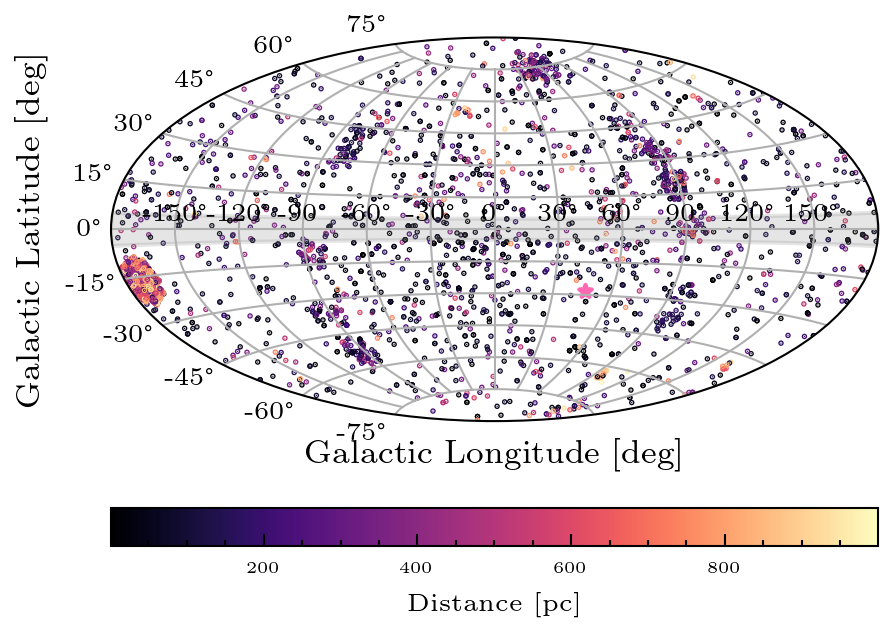
\includegraphics[width=0.6\textwidth]{figures/galactic_projection_NEA.png}
%     \caption{Some plot here with target of intrests that fall within the zenith pointings and their associated Jy measurements based on Tsys etc. }
%     \label{fig:enter-label}
% \end{figure}

\subsection{Operation's Research}
By operating a telescope on the moon, there is a wealth of information that can be gathered scietifically and about the engineering. Through this we can answer questions such as:

\begin{itemize}
    \item The lunar surface topography, conductivity, radiation, and bounce back of radiation and its impact on the scientific results.
    \item We can learn how to do astronomy from the moon and its challenges scientifically. 
    \item How long could the equipment last in the environment? What is the limiting factor for this?
\end{itemize}

\subsection{Science Summary}
%--What is the simplest system we could do science with.  etc.\\
%--Science verification
\subsubsection{Minimum System for Science}
The strength of a lunar farside telescope lies in its ability to uncover the unknown. It is certain that discoveries will be made regardless of the final system design, away from the influence of RFI and the ionosphere. However, depending on the final system design a number of science goals can be completed, as outlined in the sections above. The following are some highlights of science that could be completed with a simpler system. 

One example is only having access to an incoherent sum. This is similar to a single-dish telescope where there is no ability to pinpoint the exact location outside the field of view of the telescope itself. The time and frequency dynamic spectrum, combined with a catalog of the sources within the field, will still provide some indication of the type of event we are seeking to study. 

Provided we continue with a multibeam array as indicated in Figure \ref{fig:midband_beam_maps}, then a range of frequency and time resolutions will provide interesting results. Experiments such as technosignature searches can take on a range of different characteristics and can be easily molded to fit the system limitations. On the other hand, searches for FRBs may require a rigid approach to detect them and their analogs. When studying the solar system, we have little experience studying our planetary neighbors at the lowest radio frequencies, but studying lightning storms and other dynamic phenomena can benefit from the highest time resolution.  

Overall, no matter what the final system design allows, wonderful new discoveries will be made.


\begin{table}
\centering
\caption{A table summarizing the requirements for each science case.}
\begin{tabular}{|l|llll|l|} 
\hline
\textbf{Science Case} & \textbf{Receiver Band} & \textbf{Freq. Res.} & \textbf{Time Res.} & \textbf{Targets}                                           & \textbf{Note}                                                                                         \\ 
\hline
Technosignature       & Low                    & 10Hz                & 0.2-0.5sec         & Gaia Stars                                                 & \multirow{3}{*}{\begin{tabular}[c]{@{}l@{}}Flexible on time and \\frequency resolution\end{tabular}}  \\
                      & Mid                    & 10Hz                & 0.2-0.5sec         & Gaia Stars                                                 &                                                                                                       \\
                      & High                   & 10Hz                & 0.2-0.5sec         & Gaia Stars                                                 &                                                                                                       \\ 
\hline
Pulsar                & Low                    & 0.5MHz              & 1ms                & Blind Search                                               & \multirow{3}{*}{Can target known pulsars}                                                             \\
                      & Mid                    & 0.5MHz              & 1ms                & Blind Search                                               &                                                                                                       \\
                      & High                   & 0.5MHz              & 1ms                & Blind Search                                               &                                                                                                       \\ 
\hline
FRB Analogs           & Low                    & 0.5MHz              & 10ms               & Blind Search                                               & \multirow{3}{*}{\begin{tabular}[c]{@{}l@{}}Need some small DM \\search in realtime\end{tabular}}      \\
                      & Mid                    & 0.5MHz              & 10ms               & Blind Search                                               &                                                                                                       \\
                      & High                   & 0.5MHz              & 10ms               & Blind Search                                               &                                                                                                       \\ 
\hline
Flare Stars           & Low                    & 0.5MHz              & 1sec               & Gaia Stars                                                 & \multirow{3}{*}{\begin{tabular}[c]{@{}l@{}}Addition of Stokes V \\enhances science\end{tabular}}      \\
                      & Mid                    & 0.5MHz              & 1sec               & Gaia Stars                                                 &                                                                                                       \\
                      & High                   & N/A                 & N/A                & N/A                                                        &                                                                                                       \\ 
\hline
Solar System          & Low                    &                     &                    & Local Planets                                              & \multirow{3}{*}{\begin{tabular}[c]{@{}l@{}}Addition of Stokes V \\enhances science\end{tabular}}      \\
                      & Mid                    &                     &                    & Local Planets                                              &                                                                                                       \\
                      & High                   & N/A                 & N/A                & N/A                                                        &                                                                                                       \\ 
\hline
Studies of the Sun    & Low                    & 0.5MHz              & 1--2ms             & Sun                                                        & \multirow{3}{*}{\begin{tabular}[c]{@{}l@{}}Addition of Stokes V \\enhances science\end{tabular}}      \\
                      & Mid                    & 0.5MHz              & 1--2ms             & Sun                                                        &                                                                                                       \\
                      & High                   & N/A                 & N/A                & N/A                                                        &                                                                                                       \\ 
\hline
HI Studies            & Low                    & N/A                 & N/A                & N/A                                                        &                                                                                                       \\
                      & Mid                    & 1kHz                & 5--8sec            & Radio Galaxies                                             &                                                                                                       \\
                      & High                   & 1kHz                & 5--8sec            & Radio Galaxies                                             &                                                                                                       \\ 
\hline
RRL                   & Low                    & N/A                 & N/A                & N/A                                                        &                                                                                                       \\
                      & Mid                    & 0.5kHz              & 5--8sec            & SNR\& HMS$^{1}$ &                                                                                                       \\
                      & High                   & 0.5kHz              & 5--8sec            &                                                            SNR\& HMS$^{1}$&                                                                                                       \\
\hline
\end{tabular}
$^{1}$HMS=High Mass Star formation regions
\end{table}


\subsubsection{Science Verification}

Whenever a new instrument or telescope is brought online, a verification that the sytem is doing what you expect is necessary. Observational radio astronomy has been going on since World War II, creating a vast catalogue of sources and their behaviour. Therefore, we can use a combination of our knowledge of such sources and simultaneous observations with other telescopes to verify the system. 

%PLOTS That could be useful 
% Frequency/Wavelength against Flux Density of Transients -> parameter space plot 
% Variation of Tsys (basically mapping galactic forground) as a function of Lunar Latitude 
% Senstivity as function of integration time 
% Galactic latitude on the x axis, sensitivity on the y, carious longitudes overlapped. 
% Galactic projection plot for areas/exoplanets of intrest, i.e. benchmarking well known targets. 
% Also worth running some numbers to see how much time A team targets are in primary 